\chapter{Contexto Geológico}
A Bacia do Paraná desenvolveu-se sobre uma área de escudo do continente Gondwana Sul e é composta por uma série de núcleos cratônicos, rodeados por vários cinturões móveis e cobertos por bacias molássicas, que foram desenvolvidas durante o ciclo termo-tectônico Brasiliano que se estendeu desde o neoproterozóico até o Ordoviciano. A deformação decorrente deste ciclo teve início entre $700$ Ma e $650$ Ma, sendo que a maior parte das intrusões de granitos que podemos observar na Bacia, situou-se dentro do limite entre o Proterozóico e o Paleozóico (cerca de $570$ Ma) com resfriamento durante o Cambro-Ordoviciano entre $500-450$ Ma \citep{zalan_p._v._tectonica_1987, hawkesworth_tectonic_2000}.

O embasamento que circunda a Bacia do Paraná é dividido em: margem Leste/Sudeste, representado pelas faixas Dom Feliciano e Ribeira ,de idade Brasiliana e de direção NE-SW, separados por um núcleo cratônico designado Rio de La Plata/ Luiz Alves; margem Norte/Nordeste, representada pela faixa Uruaçu, de idade mesoproterozóica, de direção NW e por dois maciços arqueanos (Guaxupé e Goiás) remobilizados durante o ciclo Brasiliano; margem Oeste/Noroeste representada pela faixa de dobramentos Paraguai/Araguaia, também do ciclo Brasiliano, que delimita o extremo da borda Noroeste da Bacia \citep{borghi_2002, hawkesworth_tectonic_2000}.

Dentre os principais grupos de estruturas, nota-se três grupos de lineamentos de direções preferenciais NW-SE, E-W e NE-SW, representando cada um evento termo-tectônico distinto. O conjunto de lineamentos NW-SE são os mais antigos e estão relacionados ao evento  termo-tectônico do Transamazônico, e, as zonas de falhas geológicas associadas a este evento foram reativadas durante o rifteamento do Atlântico Sul, no Cretáceo.  Os lineamentos E-W, tiveram início a partir do Triássico e são paralelos às zonas de fratura oceânica, sugerindo uma ligação com o desenvolvimento do Atlântico Sul. Os lineamentos NE-SW são derivados do evento tremo-tectônico Brasiliano e de seus cinturões móveis associados. Este último conjunto de lineamentos é isento de diques de basalto \citep{milani_outline_1999}. 

O registro estratigráfico da Bacia do Paraná é formado por pacote sedimentar e magmático de espessura máxima em torno de $7000$ m, que coincide geograficamente com o depocentro estrutural da sinéclise e com a calha do rio paraná \citep{milani_orogenias_1998}. O registro estratigráfico da Bacia do Paraná é dividido em seis unidades de ampla escala ou supersequências \citep{Vail_1977} na forma de pacotes rochosos com intervalos temporais de algumas dezenas de milhões de anos de duração e envelopados por superfícies de discordância de caráter inter-regional: Rio Ivaí (Ordoviciano-Siluriano), Paraná (Devoniano), Gondwana I (Carbonífero-Eotriássico), Gondwana II (Meso a Neotriássico), Gondwana III (Neojurássico-Eocretáceo) e Bauru (Neocretáceo). As três primeiras supersequências são representadas por sucessões sedimentares que definem ciclos transgressivos e regressivos ligados às oscilações do nível relativo do mar, durante o Paleozóico, ao passo que as demais correspondem a pacotes de sedimentos continentais com rochas ígneas associadas. As unidades formais da litoestratigrafia, quais sejam os grupos, formações e membros comumente utilizados na descrição do arranjo espacial dos estratos da bacia, inserem-se como elementos particularizados neste arcabouço aloestratigráfico de escala regional \citep{boletim_2007}.

O mapa geológico (Fig. \ref{mapa geologico}) apresenta a extensão e os limites da Bacia do Paraná \citep{Vidotti_2003}.



\begin{figure}[H]
	\centering
	\setlength{\fboxsep}{8pt}
	\setlength{\fboxrule}{0.1pt}
	\fbox{
		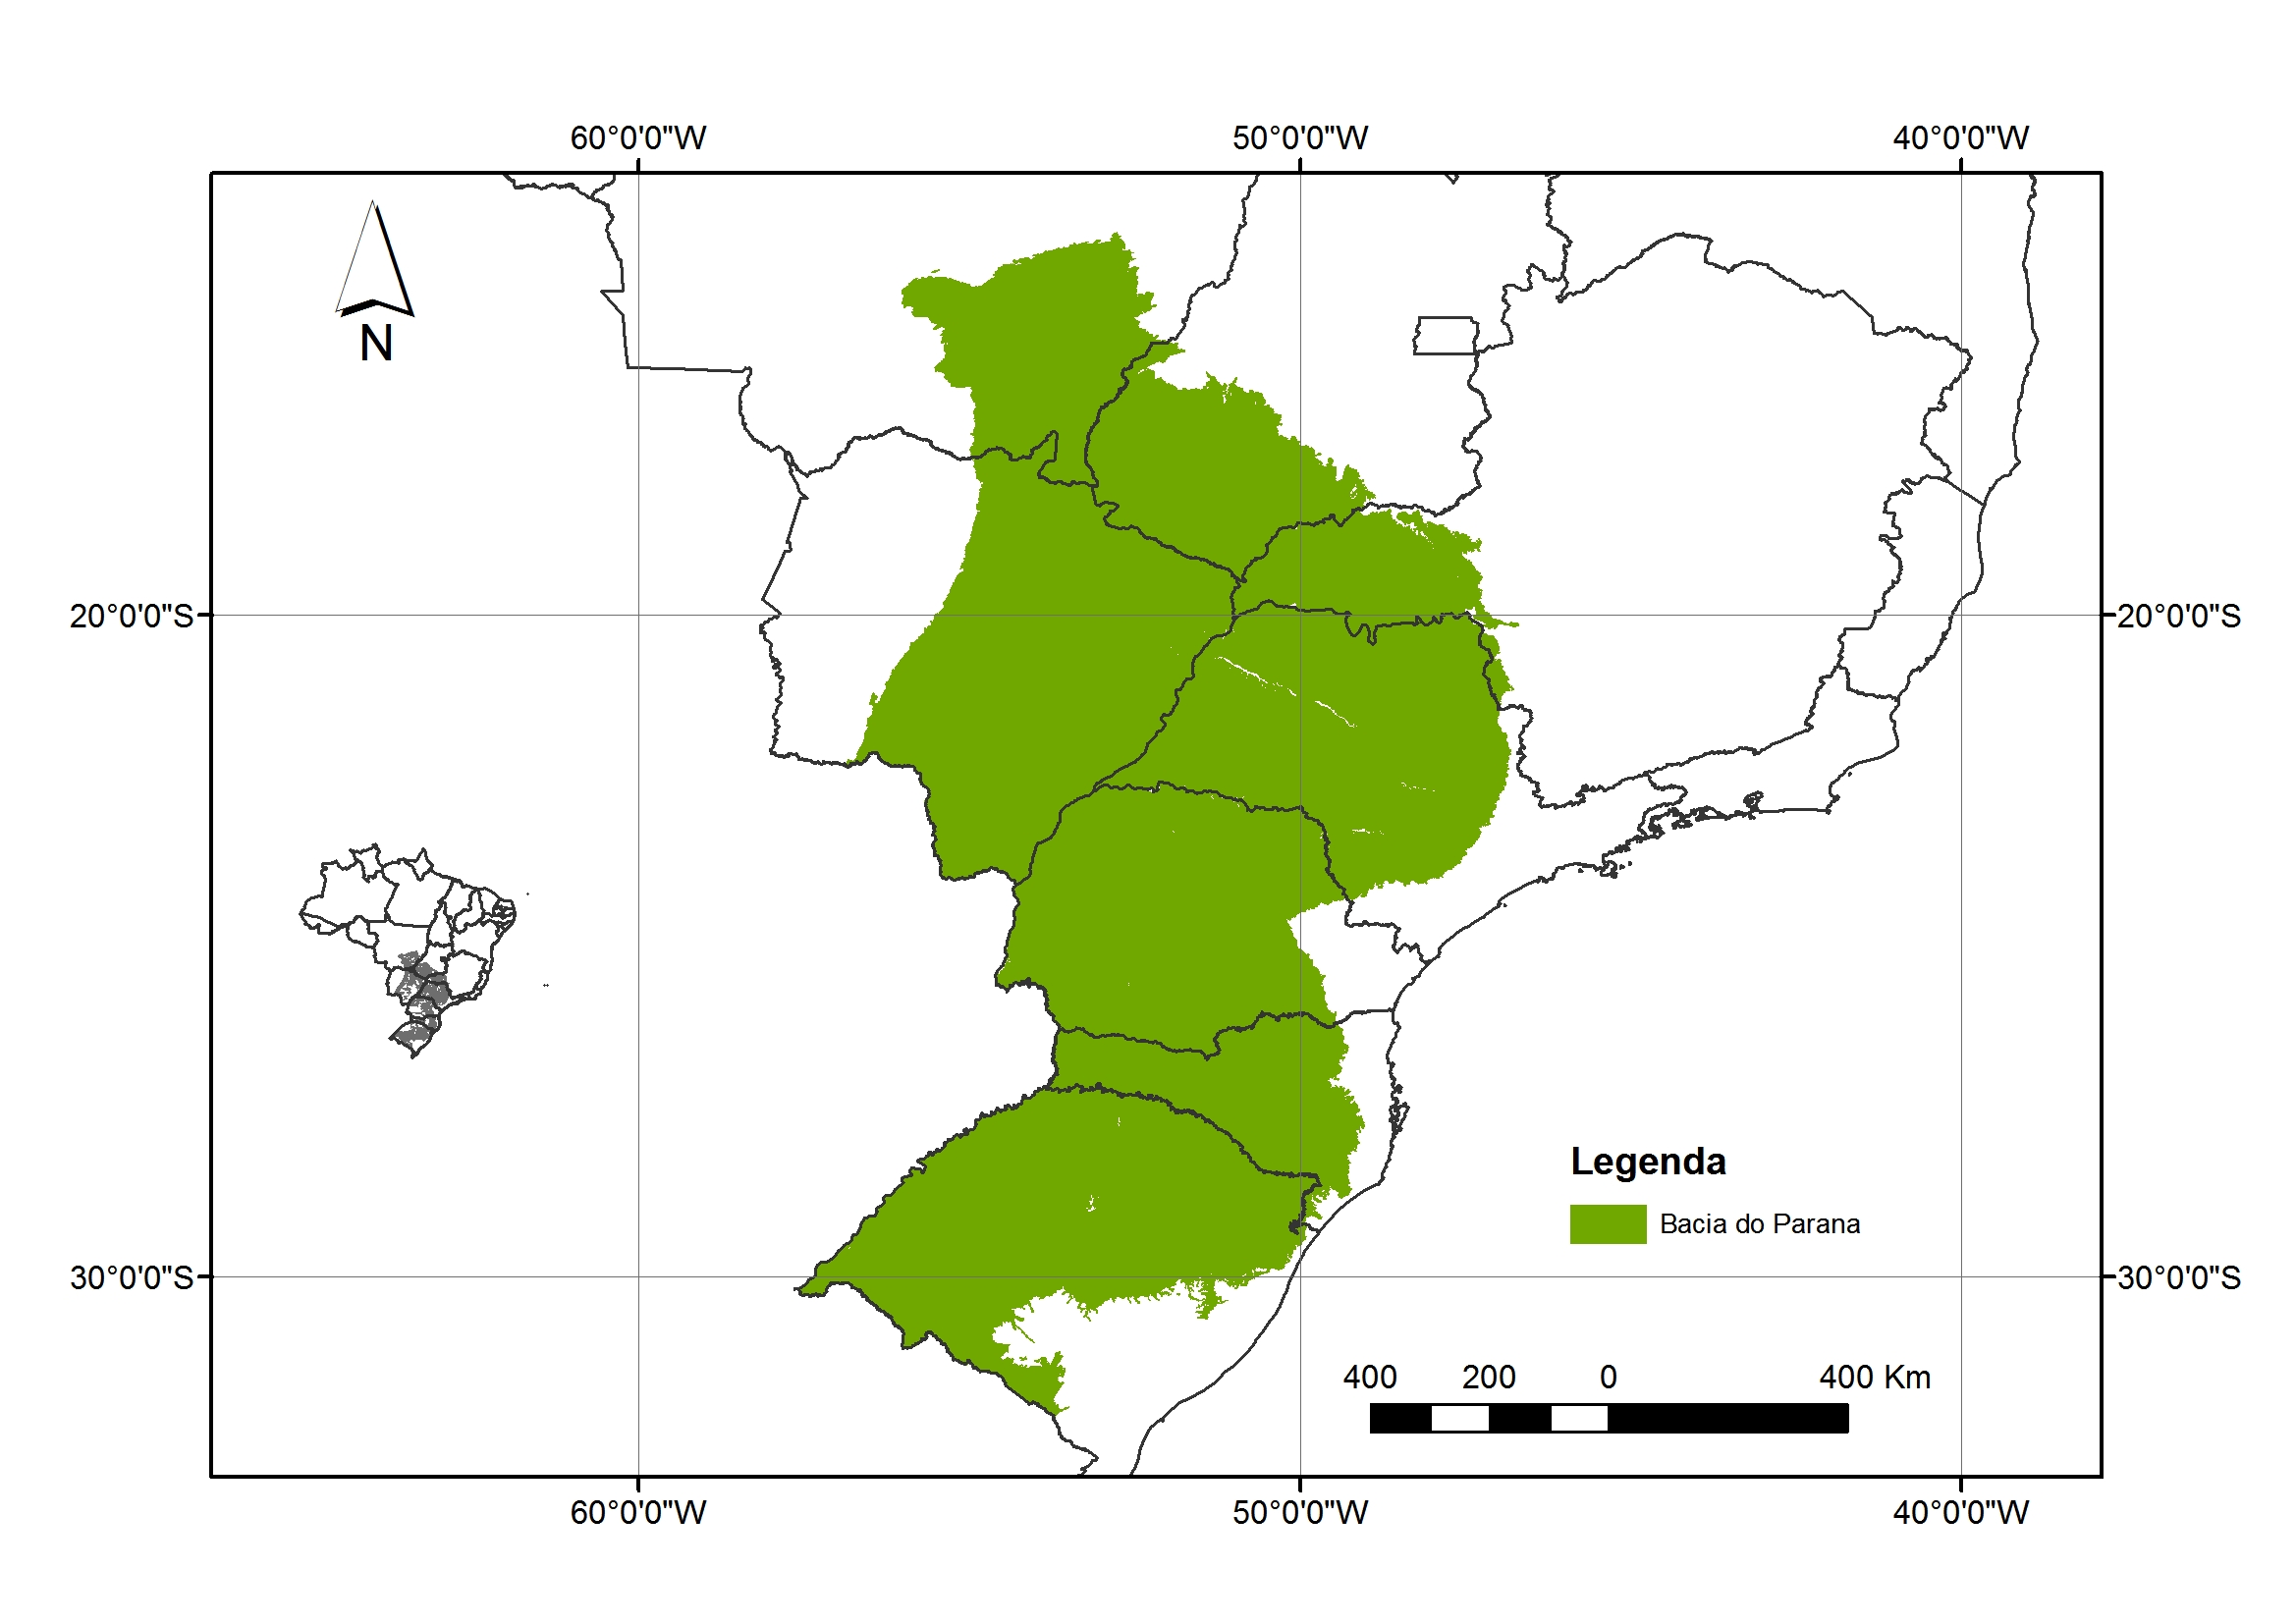
\includegraphics[scale=0.4]{Imagens/BaciaParana.jpg}
	}
	\caption{Mapa geológico e de localização da área de estudo. }
	\label{mapa geologico}
\end{figure}

